\chapter{Implementace}
\label{chap:implementation}
Celý systém pro správu kampaní je rozdělen do několika celků. Základem je webový server, který zprostředkovává komunikaci mezi různymi dalšími častmi.
Data jsou perzistována v relační databázi PostgreSQL.
Paměťové úložiště v databázi Redis slouží jako zprostředkoval pro frontu úloh, cacheování požadavků na API třetích stran a dočasné úložiště importovaných dat.

\begin{figure}[h]
    \centering
    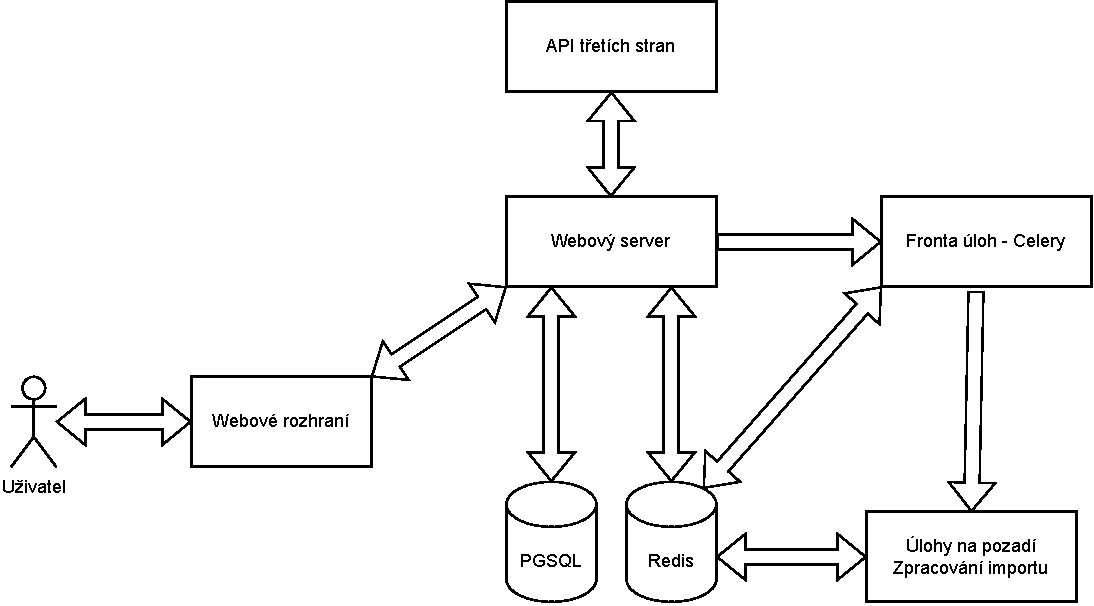
\includegraphics[width=1\textwidth]{Figures/system-overview.pdf}
    \caption{Náhled systému}
    \label{fig:system-overview}
\end{figure}

\section{Importování souborů}
Ve webovém rozhraní, které slouží jako hlavní způsob interakce systému s uživatelem, je umožněno vybírání souboru ke zpracování.
Jakmile je tento soubor nahrán na server, vytvoří se nový úkol do fronty úloh. Na pozadí je automaticky spuštěň nový proces, který
zpracovává nahraný soubor. Uživatele v tento moment nic neblokuje a nebrání s další interakcí se systémem. Jakmile jsou data ze souboru
získána, jsou dočasně uloženy do paměťové databáze Redis a uživateli je zobrazeno upozornění.
Po rozkliknutí je přesměrován na stránku, kde si může vybrat, které části si přeje importovat a které ne.
V případě využití funkce najít a nahradit se spustí další úloha na pozadí, která tento požadavek splní.
Následně jsou data zapsaná do relační databáze.

% Dodělat do systému funkci najít a nahradit -> další celery task, který upraví data, přepíše v 
% Redisu a pošle request na Webserver, který to už uloží do DB

\section{Tabulková správa kampaní}

\subsection{Návrhy klíčových slov}

\section{Export kampaní}


\endinput